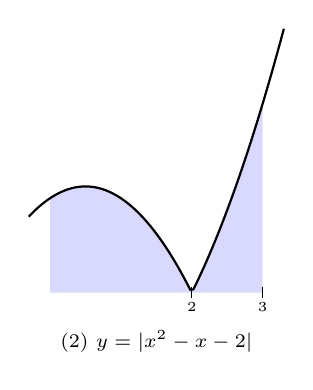
\begin{tikzpicture}[x=9mm,y=6mm]
\fill[blue!15] plot[domain=0:3,samples=60] (\x,{abs((\x)^2-\x-2)}) -- plot[domain=3:0,samples=60] (\x,{0}) -- cycle;
\ax{-0.5}{3.5}{-0.5}{4.6}
\draw[thick,domain=-0.3:3.3,samples=80] plot (\x,{abs((\x)^2-\x-2)});
\draw (2,0.12)--(2,-0.12); \node[below] at (2,0){\tiny $2$};
\draw (3,0.12)--(3,-0.12); \node[below] at (3,0){\tiny $3$};
\node[below] at (current bounding box.south){\scriptsize (2) $y=|x^2-x-2|$};
\end{tikzpicture}